%\documentclass[10pt,a4paper]{scrreport}
\documentclass[10pt,a4paper]{scrarticle}
%müssen wir scrreport nehmen?
%scrreport braucht als obereinheit chapter nicht sections, deswegen 0.1,0.2 etc
\usepackage{hyperref}
\usepackage[utf8]{inputenc}
\usepackage[T1]{fontenc}
\usepackage[ngerman]{babel}
\usepackage{amsmath}
\usepackage{amsfonts}
\usepackage{amssymb}
\usepackage{graphicx}
\usepackage{imakeidx}
\usepackage{todonotes}
%\usepackage[hyphens]{url}
\usepackage{natbib}
\bibliographystyle{alpha}

\makeindex
\title{Ein Kameragestützer linearer Encoder für Seile}
\author{Bruno Reinhold, Felix Fleisch}

\begin{document}
	\maketitle
	\newpage
    %\printindex
    \tableofcontents
\section{Einführung}
Heutzutage übliche lineare Encoder Systeme, welche auf optischen Verfahren basieren, sind oftmals teure Hochpräzisionsinstrumente. Diese Systeme bieten Auflösungsgenauigkeiten bis in den Bereich von Nanomenter. Lineare Encoder, welche für Seile geeignet sind und eine geringere Genauigkeit voraussetzen sind eher unüblich. Mit dieser Arbeit wollen wir daher zeigen, dass sich ein linearer Encoder mit einfacher Hardware und bewährten Methoden des Rechnersehens umsetzen lässt.

%wohin das abstract
\subsection{Zielsetzung}\label{Zielsetzung}
Ziel der Arbeit ist es eine Python-Bibliothek zu entwickelt, um eine an den Rechner angeschlossene Kamera als linearen Encoder benutzen zu können. Hierzu wird ein neuer Algorithmus entwickelt. Dieser soll sequentiell für eine Folge von Bildern, das Muster auf dem Seil benutzt, um diskrete Perioden zu zählen und eine Abweichung von der Startposition auszugeben. %awkward
Dies macht es einfach, eine geschlossene Regelschleife und genaue Positionierung für verschiedenste Anwendungen zu erstellen.
Die Bibliothek und der Entwicklungsprozess sollen gut dokumentiert werden.
Die entwickelte Methode soll ausführlich unter verschiedenen Bedingungen getestet werden.


\subsection{Motivation}\label{Motivation}
Ein linearer Encoder ist ein Messgerät, mit welchem die Distanz entlang einer Achse gemessen werden kann. Klassischerweise wird hierfür eine optisch oder magnetisch markierte Schiene benutzt, welche bei Bewegung eine Signaländerung in einem Sensor hervorruft. Das Signal kann interpretiert werden, um eine Distanz zu erhalten. Hierbei unterscheidet man \textit{inkrementelle} und \textit{absolute} Encoder. Ein absoluter Encoder verschlüsselt seine Position im Signal, während ein inkrementeller Encoder die Position aus diskreten Signaländerungen aufsummiert. Sie werden benutzt, um eine genaue Positionierung von verschiedener Hardware, wie z.\,B. CNC Maschinen zu erlauben.

\begin{figure*}[!b]
+  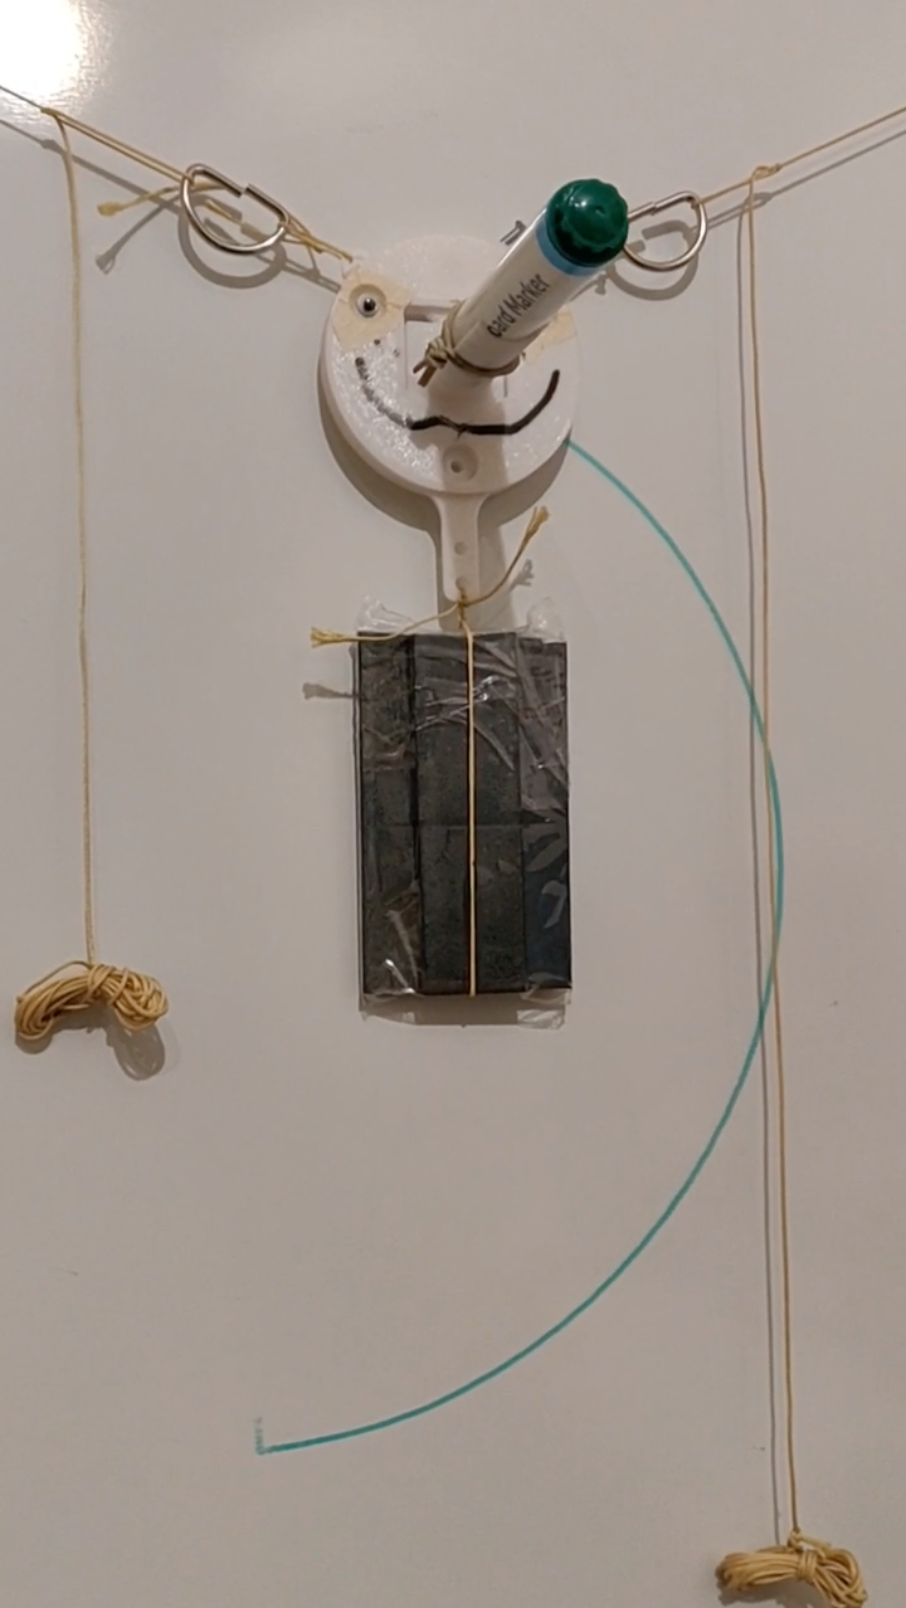
\includegraphics[scale=0.3]{Abbildungen/2D_plotter.png}
  \centering
  \caption{Das Kopfteil eines 2D V-Plotters, der einen Halbkreis auf ein Whiteboard zeichnet.}
  \label{fig:2D_plotter}
\end{figure*}

Ein Seilantrieb ist ein Antrieb, in welchem ein Seil mit einem Motor bewegt wird, um z.B. einen V-Plotter zu positionieren, wie in Abbildung \ref{fig:2D_plotter} zu sehen ist. Seilantriebe sind preisgünstig und mechanisch einfach. Die Länge des Seils lässt sich außerdem fast beliebig skalieren. Seilantriebe mit einfachen Rollen sind inhärent über lange Zeiträume ungenau, was eine offene Regelschleife unzuverlässig macht. Dies wurde experimentell im Voraus festgestellt. Es wurde ein ähnlicher Fehler für einen mit einer Rolle am Seil angetrieben Magnet-Drehgeber festgestellt.

Eine Hypothese dafür, wie dieser Fehler auftritt, ist wie folgt: jedes Seil ist zu einem gewissen Grad dehnbar. Vor und hinter dem Antrieb ist unterschiedlich viel Spannung auf dem Seil, weshalb 
das Seil auf einer Seite des Motors weiter gedehnt ist. Dies resultiert daraus, dass bei einer gleich großen Vorwärts- und Rückwärtsbewegung auf der einen Seite mehr Seil aufgenommen wird als abgegeben. Der Motor kehrt an seine ursprüngliche Position zurück, das Seil hat sich jedoch bewegt, ohne je durchzurutschen.

Um dies zu verhindern, kann das Seil durch einen Zahnriemen oder z.\,B. eine Gardinenkette ersetzt werden, welche mechanisch mit dem Antrieb verschränkt ist und somit nur diskrete Fehler zulässt. Dies verhindert ein allmähliches Abwandern.

Alternativ kann eine geschlossene Regelschleife benutzt werden, um den sich langsam ansammelnden Fehler zu messen und laufend zu korrigieren. In diesem Projekt wurde mit einer Webcam ein Seil gefilmt und seine diskreten Markierungen benutzt, um Information über die zurückgelegte Strecke zu erhalten. Die Benutzung eines Seils ist vorteilhaft, da Seile günstiger zu beschaffen sind und die entsprechenden Umlenkrollen viel einfacher gestaltet werden können.

%done-vorteile alternative (billig)

%bruno inhalte aus den dokus integrieren



\subsection{Literatur}
    Wir haben den Algorithmus Shift-Detection by Restoration, der im Paper von Suesse et al. \cite{suesse1999shift} beschreiben wird, benutzt um die Phase des Seiles zu berechnen. Darüber hinaus haben wir in unserer Recherche zur Benutzung von Kameras als lineare Encoder, keine weiteren direkt relevanten Arbeiten gefunden.
	%paper shift detection by restoration
	%andere theorie?

\section{Theorie}
    In diesem Kapitel werden die theoretischen Grundlagen behandelt, welche dem linearen Encoder zugrunde liegen. Dies beinhaltet eine theoretische Betrachtung der Region-of-Interest (RoI) sowie die theoretischen Grundlagen der beiden implementierten Ansätze für die Verschiebungsbestimmung: zum einen mithilfe von Kreuzkorrelation zum anderen mithilfe von Restauration.
    %grober überblick funktion
    %kann man in theorie implementation mit beschreiben? ich weiß es nicht
    %bruno: habe jetzt eine extra section dafür gemacht    
    
	\subsection{Extraktion der RoI}\label{RoI_Extraktion}
	Bevor der lineare Encoder mit der Bestimmung der Verschiebungsdistanz beginnen kann, muss zunächst eine RoI bestimmt werden. Dies bedeutet, dass die ursprünglichen Videoframes auf eine zentrale  Region, welche nur das Seil zeigt, zugeschnitten werden. Die Extraktion der RoI beinhaltet drei aufeinander folgende Arbeitsschritte. Zuerst wird mittels des Canny-Edge-Detection Algorithmus der Umriss des Seils sowie dessen Muster bestimmt, um anschließend durch die detektierten Kanten mittels der Hough-Transformation die Lage des Seils im Videoframe zu bestimmen. Der dritte Schritt nutzt dann die mit der Hough-Transformation bestimmten Linien, um die Breite zu erkennen und die RoI in der Mitte des erkennbaren Seils auszuschneiden. 

\begin{figure*}
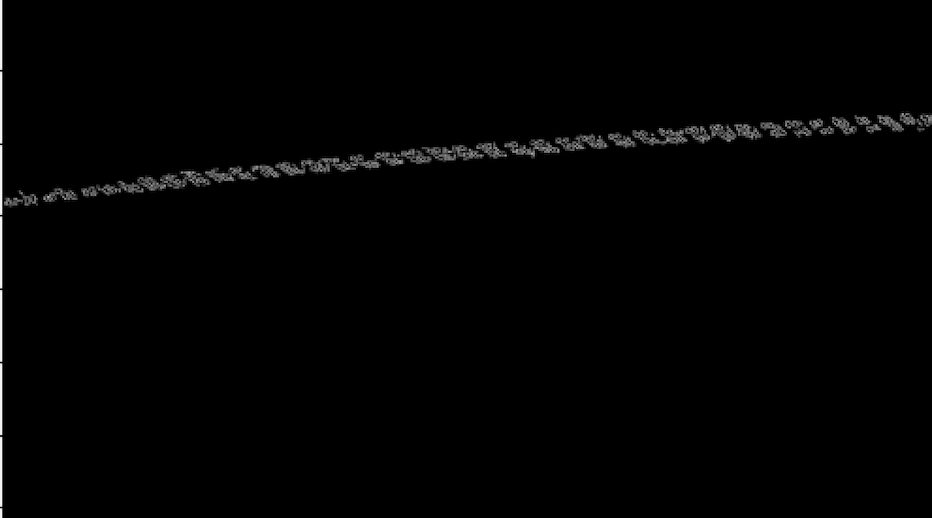
\includegraphics[width=10cm]{Abbildungen/cannyEdges.png}
  \centering
  \caption{Kantenbild, das aus dem Canny-Algorithmus resultiert.}
  \label{fig:CannyEdges}
\end{figure*}

		\subsubsection{Canny-Edge-Detector}\label{CannySubsection}
		Der Canny Algorithmus zur Kantenerkennung wurde von John F. Canny entwickelt und eignet sich hervorragend, um die Kanten des Seils zu finden 		\cite{canny_computational_1986}. Der Canny Algorithmus besteht dabei aus vier Phasen.\\ 
		Die erste Phase ist eine simple Rauschreduktion, welche mit der Faltung eines $5\times5$-Gauss-Filters erreicht wird.\\
	    Das Ziel der zweiten Phase ist das Finden der Intensitätsgradienten. Die Gradienten des geglätteten Bildes werden in horizontaler und vertikaler Richtung durch die Anwendung eines Sobelfilters berechnet. Ausgehend von den Gradienten in der horizontalen Richtung $G_x$ und der vertikalen Richtung $G_y$ lassen sich für jedes Pixel der Kantengradient mit \\
	    \begin{equation}
        G_{gradient}=\sqrt{G^2_x + G^2_y}
        \end{equation}
        und die entsprechende Richtung mit\\
        \begin{equation}
        \Theta=tan^{-1}\left(\frac{G^2_x}{G^2_y}\right)
        \end{equation} bestimmen.
        Die Kanten verlaufen immer senkrecht zum Gradienten. Allerdings wird die  Gradientenrichtung in der Praxis auf die vertikale, horizontale oder diagonale Achse gerundet.\\
        Die dritte Phase nennt sich Non-Maximum Suppression, deren Ziel es ist, alle Pixel zu finden, die für eine Kante in Frage kommen. Es entsteht damit ein Bild, auf dem die Kanten des Bildes schon in Ansätzen zu sehen sind. Dieser Zwischenschritt wird erreicht, indem alle Pixel des Gradientenbilds, welche bezogen auf eine Gradientenrichtung kein Maximum in der lokalen Nachbarschaft darstellen, auf null gesetzt werden.\\
        Die vierte und letzte Phase besteht aus der Anwendung einer Hystereseschwellwertoperation. Diese ist notwendig, um zu entscheiden, welche der vorher bestimmten Kantenkandidaten tatsächlich Kanten sind. Dazu werden zwei Schwellwerte definiert, ein unterer Schwellwert $threshold_{min}$ und ein oberer Schwellwert $threshold_{max}$. Alle Kanten, deren Pixelwerte vollständig unter $threshold_{min}$ liegen sind sicher keine Kanten und alle Pixelwerte welche über $threshold_{max}$ liegen sind definitiv Kanten. Für Kantenpixel, welche zwischen den beiden Schwellwerten liegen, entscheidet deren Verbindung zu anderen Kantenpixel. Ist ein Pixel, welches unter zwischen $threshold_{min}$ und $threshold_{max}$ liegt, mit einem Pixel verbunden, welches über $threshold_{max}$ liegt, ist diese Pixel endgültig Teil der Kante, andernfalls wird es ebenfalls auf Null gesetzt.\\
        Das Ergebnis ist ein Binärbild, bei dem alle Nicht-Kantenpixel den Wert Null haben und alle Kanten dem Maximalwert entsprechen, wie in Abbildung \ref{fig:CannyEdges} zu erkennen ist. 
        
\begin{figure*}
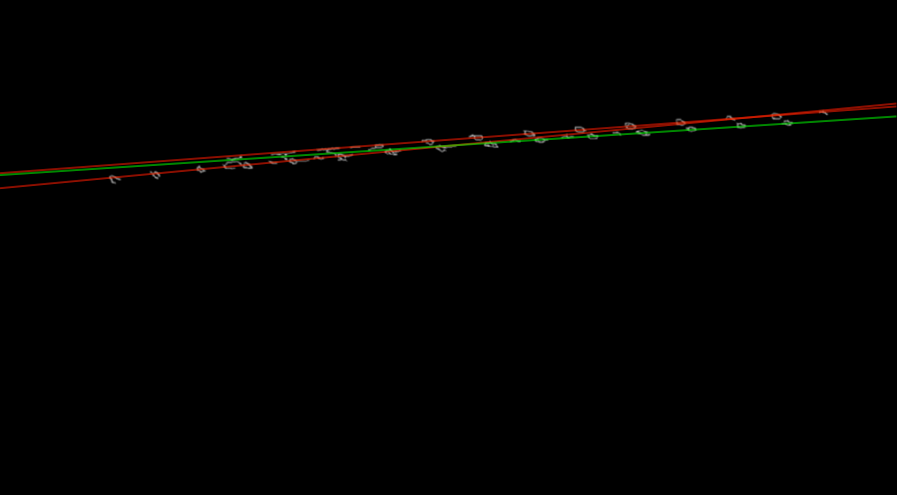
\includegraphics[width=10cm]{Abbildungen/rope_houghLines.png}
  \centering
  \caption{Mithilfe des Kantenbildes lassen sich Hough-Linien berechnen. Die roten Linien stellen beispielhaft berechnete Hough-Linien dar. Die grüne Linie stellt die berechnete durchschnittliche Linie dar.}
  \label{fig:HoughLinien}
\end{figure*}
        
		\subsubsection{Hough-Transformation}\label{Hough_Transformation}
		Mit der Hough-Transformation lassen sich Geraden für ein Bild berechnen, welche durch die annähernd geraden Kanten eines Bildes verlaufen \cite{toennies2005grundlagen}. Als Eingabe verwendet der Algorithmus das in \ref{CannySubsection} berechnete Kantenbild. Die Geradenberechnung wird für jeden Kantenpunkt $(x,y)$ durchgeführt, wobei sich eine Schar von Geraden in Polarkoordinaten über die Gleichung
		\begin{equation}
        r_{\Theta}=x\cdot\cos{\left(\Theta\right)}+y\cdot\sin{\left(\Theta\right)}  
        \end{equation}
        ergibt. Diese wird auf ein Sinusoid im Intervall von $0\leq r\leq d$ und $0^\circ\leq\Theta\leq180^\circ$ beschränkt, da sich so alle möglichen Geraden im Kantenbild darstellen lassen. Einen diskretisierten Parameterraum, der durch das Intervall beschränkt ist, nennt man Hough-Array. Punkte einer Gerade im Kantenbild entsprechen im Hough-Array einem Schnittpunkt der entsprechenden Sinusoide. Demzufolge sucht man im Hough-Array nach Punkten, in denen sich möglichst viele Sinusoide schneiden. Eine Gerade im Kantenbild wird erst dann definiert, wenn ein Schwellwert erreicht wurde, der festlegt, wie viele Sinusoide sich in diesem Punkt schneiden müssen. Der Schwellwert legt also die minimale Anzahl an Schnittpunkten im Hough-Array fest, die benötigt wird, um eine Gerade im Kantenbild zu detektieren. Die Lage des Seils wird nun mithilfe einer von mehreren Hough-Linien gemittelten Linie approximiert. Abbildung \ref{fig:HoughLinien} zeigt die roten Linien, welche beispielhaft die Hough-Linien mit den meisten Schnittpunkten im Hough-Array darstellen. Die grüne Linie ist die aus den roten Linien gemittelte Hough-Linie, welche die Lage des Seils bestmöglich repräsentieren soll. Dies ist nur möglich, weil nur ein Seil im Bild vorhanden ist.
        
\begin{figure*}
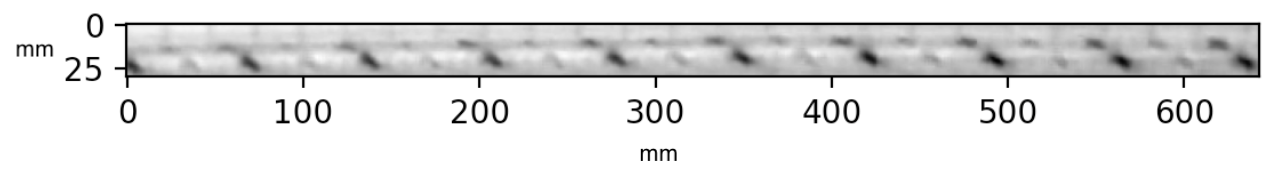
\includegraphics[width=10cm]{Abbildungen/RoI_scales.png}
  \centering
  \caption{Die RoI zeigt die für die Verschiebungserkennung notwendigen Markierungen des Seils.}
  \label{fig:RoI_img}
\end{figure*}
    

\begin{figure*}
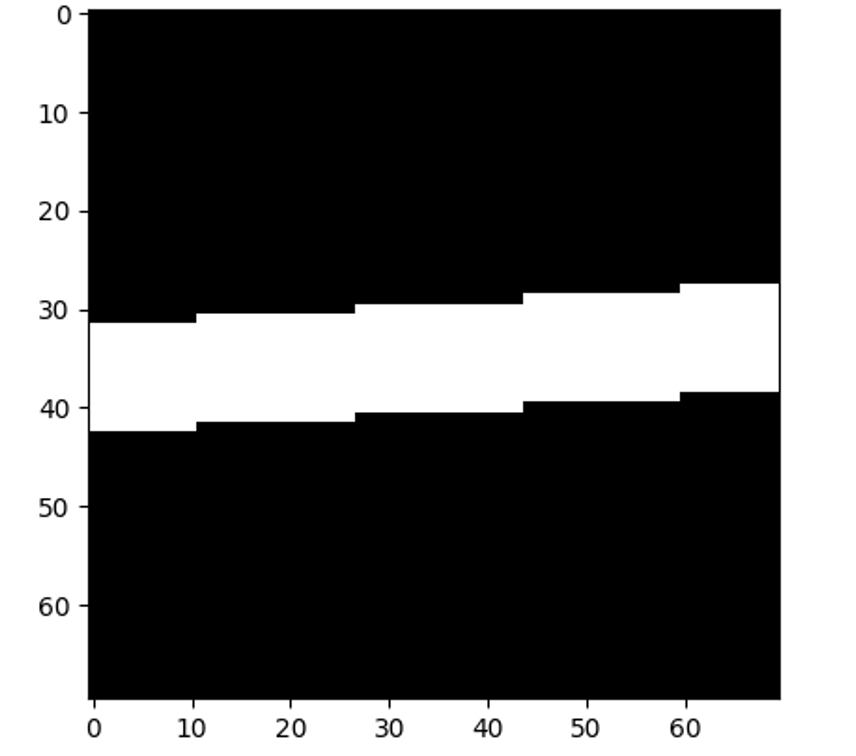
\includegraphics[width=10cm]{Abbildungen/filterMask.png}
  \centering
  \caption{Eine Filtermaske.}
  \label{fig:filtermaske}
\end{figure*}

		\subsubsection{Ausschneiden der RoI}\label{RoI_Ausschneiden}
		Das Fenster für die RoI wird nun in der Mitte des Seils mittels des Kantenbildes, einer Maske und der mittleren Hough-Linie gebildet. Zunächst wird mithilfe des Kantenbildes und der in Abbildung \ref{fig:filtermaske} dargestellten Maske des Seils die Breite des Seils bestimmt. Hierfür wird zuerst die Maske erzeugt, indem eine Linie in der bereits bestimmten Richtung in ein leeres Bild gezeichnet wird. Das Falten mit dieser Maske verwischt nun entlang dem Seil, aber nicht senkrecht zu ihm. Dies hat den Effekt, dass die vielen kleinen Flecken, welche durch den Canny Filter gewonnen wurden, alle in eine breite Linie verschmelzen. Nun kann von der Mitte der Linie aus pixelweise auswärts gewandert werden, bis schwarz gefunden wird. Dies gibt die Breite an.
		
		Die Mitte des Seiles wird als Mittelwert der zwei Schnittpunkte der Linie mit dem Bildrand. Der Abstand dieser zwei Randpunkte, die Breite der Linie, der Mittelpunkt und der Winkel dienen als Information um die RoI zu extrahieren.
		Um nun für ein beliebiges Bild die RoI zu bestimmen, wird das Bild zuerst um den Winkel um den Mittelpunkt gedreht. Anschließend werden Höhe und Breite zugeschnitten. Die RoI zeigt jetzt nur noch die für die Bestimmung der Verschiebung benötigten periodischen Markierungen des Seils, wie in Abbildung \ref{fig:RoI_img} dargestellt. 
		%done-genauer breitenbestimmung ergänzen
		
		
	\subsection{Bestimmung der Verschiebung}
	In diesem Abschnitt sind die theoretischen Grundlagen der beiden Verschiebungserkennungsmethoden Autokorrelation und Shift-Detection-by-Restauration (Verschiebungserkennung durch Restauration), sowie die für die Distanzberechnung notwendige Bestimmung der Periode und das Phase-Unwrapping dargelegt.
	Beide Methoden benutzen ein Referenzbild, auf welches sich alle gemessenen Verschiebungen beziehen. Hiermit wird das graduelle Ansammeln von Fehlern verhindert. Für den gesamten Operationszeitraum wird ein anfangs aufgenommenes Referenzbild benutzt, deshalb muss die Methoden besonders robust gegenüber Beleuchtungsänderungen sein. Sie bestimmen jeweils eine Verschiebung in Pixeln, welche mit der Methode des Phase-Unwrappings weiter interpretiert wird.

        
\begin{figure*}
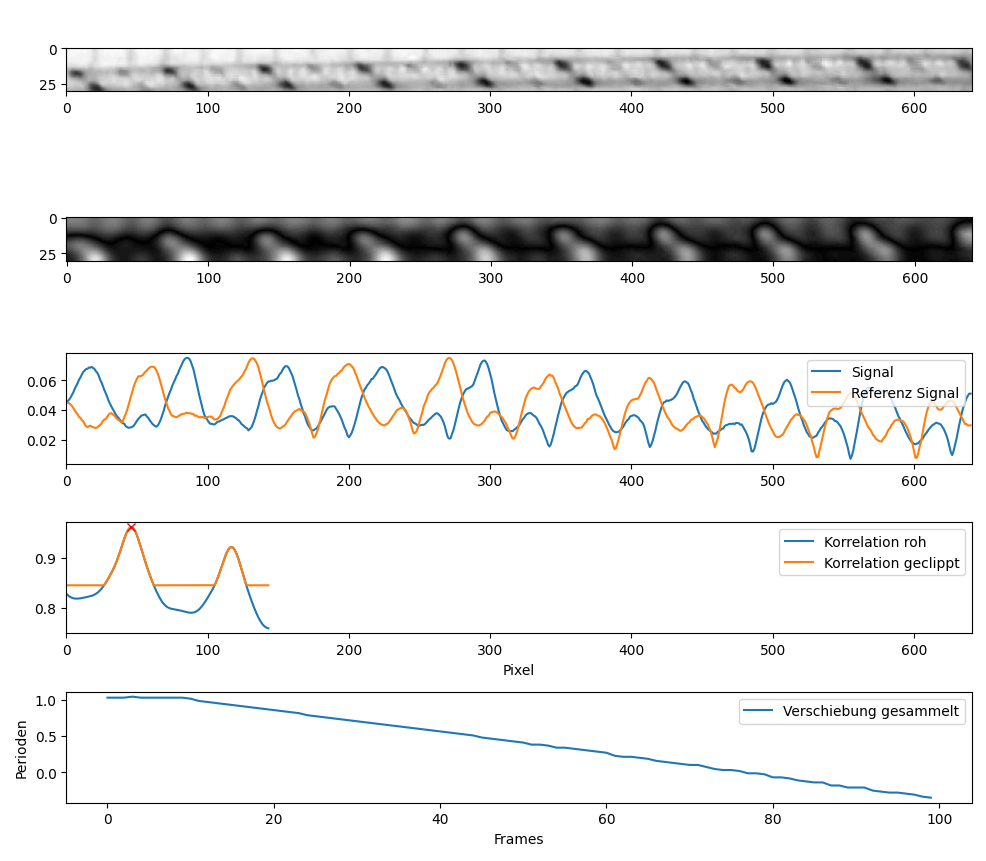
\includegraphics[width=10cm]{Abbildungen/Correlation_figure.png}
  \centering
  \caption{Die Verschiedenen Schritte in der Verschiebungserkennung mit Korrelation}%bild/caption ändern
  \label{fig:correlation}
\end{figure*}

		\subsubsection{Verschiebungserkennung mittels Autokorrelation}\label{Autokorrelation}
		%Felix
		Unser erster Ansatz für die Berechnung der Verschiebungserkennung basiert auf der Korrelation $f\circ g$, auch Kreuzkorrelation genannt. Diese wird wie folgt berechnet: an der Stelle $n$ wird sie als ein um $n$ verschobenes Skalarprodukt von $f$ und $g$ interpretiert werden. Somit lässt sich sehen, dass, wenn $g$ verschoben um $n$ mit $f$ übereinstimmt, der Wert der Kreuzkorrelation maximal wird. Die Idee ist dabei, das Maximum der Kreuzkorrelation und damit die Verschiebung mit bester Übereinstimmung von Referenz und aktuellem Bild zu bestimmen.
 		\begin{equation}
		    (f\circ g)_n=\sum_i f_{\left(n+i\right)}g_{\left(i\right)}\\
		\end{equation}
		%\begin{equation}\label{cross_correlation_2d}
        %    (f\circ g)_{m,n}=\sum_k \sum_l f_{m+k,n+l}g_{k,l}\\
		%\end{equation}
		Dazu wurde die eindimensionale Variante der Kreuzkorrelation benutzt, welches eine Vorverarbeitung des Signals voraussetzt . Zuerst wurde ein adaptiver Kantenfilter benutzt, um Belichtungsschwankungen auszugleichen. Hierzu wird die absolute Differenz zweier Gauß Glättungen berechnet. Dies ist in der zweiten Zeile von Abbildung \ref{fig:correlation} zu sehen. Um nun ein eindimensionales Signal zu erhalten, wird jede Spalte aufsummiert. Dies resultiert in dem orangenen Graphen in der dritten Zeile von Abbildung \ref{fig:correlation}.
		
		Da man einen endlichen Definitionsbereich habt, wird das Signal im Vergleich zum Referenzsignal um 2,5 Perioden gekürzt. Wenn nun die Kreuzkorrelation berechnet wird, sodass das zweite Signal vollständig in der Referenz liegt, ergibt sich ein Ergebnis der Länge 2,5 Perioden. Dieses wird geglättet und um die Erkennung von Maxima in Tälern zu verhindern, wird alles unter dem Durchschnitt des Ergebnis abgeschnitten.
		%geklippt?
		Nun wird das erste lokale Maximum bestimmt und der Index wird als Verschiebung an das Phase-Unwrapping weitergegeben. Dies ist in Abbildung \ref{fig:correlation} im mittigen Diagramm zu sehen.
		
		\subsubsection{Bestimmung der Periode}
		Für den Algorithmus des Phase-Unwrapping ist es wichtig, dass man die Periode des Signals in Pixeln kennen. Hierfür wurden zwei verschiedene Ansätze benutzt.
		Der erste bestimmt die Periode aus dem eindimensionalen Signal, welches in Abschnitt \ref{Autokorrelation} gewonnen wurde. Hierzu wird die Fouriertransformation der Helligkeitskurve des Referenzbildes berechnet. Nun wird der Index des Fourierkoeffizienten mit maximalem Betrag bestimmt, ausgenommen dem nullten Koeffizienten. Die zugehörige Wellenlänge wird aus dem Index und der Breite des Fensters berechnet und als Periode zurückgegeben.
		
		Wenn man, wie in Abschnitt \ref{Shift_detection_by_Restoration} beschrieben, Shift-Detection durch Restauration durchführt, sind für das Referenzbild $h$, bereits $\alpha_k(h)$ und $\overline{\alpha_k(h)}$ berechnet. Da sich die Korrelation $f\circ g$ auch als Faltung mit dem gespiegelten $f*g^R$ darstellen lässt und die Spiegelung im Ortsraum dem komplex konjugieten im Frequenzraum entspricht, lässt sich mithilfe des Faltungstheorems (\ref{faltungstheorem}) zeigen, dass $\alpha_k(f\circ g)=\alpha_k(f)\overline{\alpha_k(g)}$ gilt. 
		Mit einer inversen fast Fourier transform (IFFT) können wir aus $\alpha_k(h)\overline{\alpha_k{h}}$ die Autokorrelation bestimmen.
		%bild autokorrelation
		
		Wir ignorieren nun Verschiebungen in der Y-Achse, um ein eindimensionales Signal zu bekommen. Die Autokorrelation ist an der Stelle $x$ maximal, wenn das Signal verschoben um $x$ am besten mit dem Original übereinstimmt. Dies ist immer bei einer Verschiebung von $x=0$ der Fall. Lokale Maxima sagen aus, dass an dieser Stelle eine Änderung von $x$ die Übereinstimmung verschlechtern würde. Dies ist vor allem der Fall, wenn das Signal um eine Periode verschoben ist.
		Man wendet einen kleinen Gauss-Filter an, um das Signal zu glätten. Anschließend wird eine geglättete Version des Signals subtrahiert, um in einer Art Kantenerkennung nur die Spitzen hervorzuheben. Alle Werte unter dem Mittelwert werden auf den Mittelwert gesetzt. Dies dient dazu, kleine Maxima innerhalb von Tälern zu eliminieren. Zurückgegeben wird dann die Periode als Index des ersten gefundenen lokalen Maximums.
		
        Empirisch funktionieren beide Methoden gut, auch wenn es ein anderes Seil als Eingabe benutzt wird. Die Genauigkeit der Periode ist nicht kritisch. Sie kann nur einen Fehler zum Endergebnis beitragen wenn das Phase-Unwrapping fehlschlägt, weil es falsch entschieden hat. Dies senkt geringfügig die effektive Höchstgeschwindigkeit. Der andere Weg wie sich Fehler durch eine falsche Periode ins Endergebnis finden können, ist durch die Berechnung des nicht diskreten Anteils der bewegten Länge. Dieser wird aus der Phase im Bild und der Länge der Periode berechnet und hat einen Wert von null bis eins, daher ist der absolute Fehler klein.
		%beide Methoden bwewreten, klappen gut.
		
		%Felix
		%bild signal gefiltert/ungefiltert
		
		\subsubsection{Phase-Unwrapping}
        %Felix
        Wenn wir erfolgreich die Verschiebung zwischen dem Referenzbild $h$ und dem verschobenen Bild $g$ bestimmt haben, müssen wir diese Phase noch interpretieren. Hierzu benutzen wir einen naiven Ansatz zum Phase-Unwrapping, welcher trotzdem gute Ergebnisse erzielt.
        
        \begin{figure*}
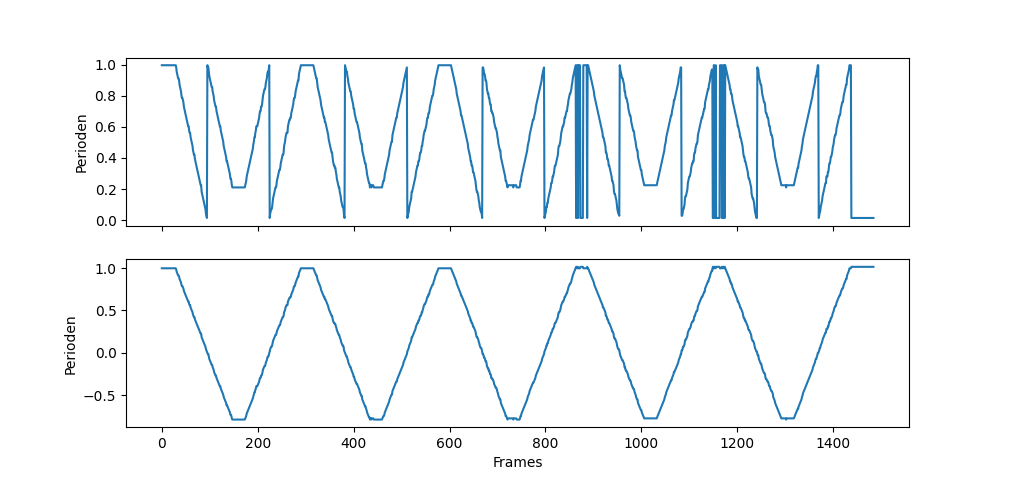
\includegraphics[width=10cm]{Abbildungen/Phase_Unwrapping.png}
  \centering
  \caption{Gemessene Phase und rekonstruierte Bewegung}%bild/caption ändern
  \label{fig:phase_unwrapping}
\end{figure*}

        Wir haben als Eingabe die Phase unserer Verschiebung bezogen auf das Referenzbild und die letzte Phase. Bewegt sich die neue Phase mehr als eine Periode, so macht sie einen Sprung. Wir erkennen einen Sprung als zwei aufeinander folgende Werte die mit einer Länge $s\geq \frac{p}{2}$ von mehr als einer halben Periode $p$ auseinander liegen. Diese Fälle können auf zwei Arten interpretiert werden: entweder können sie durch einen Sprung der Länge $s$ in Richtung $s$ oder der Länge $p-s$ entgegen der Richtung von $s$ entstanden sein.
        Diese Möglichkeiten lassen sich nicht unterscheiden. Weil wir von einer langsamen Geschwindigkeit ausgehen, wird immer der zweite Fall angenommen. Hieraus ergibt sich eine maximale Geschwindigkeit, über welche der Algorithmus nicht mehr funktioniert.
        Wir verwalten zusätzlich eine Variable, in welcher die totale Anzahl der Sprünge entsprechend der Perioden verwaltet wird. Diese wird in Abhängigkeit von der Richtung des Sprunges geändert. Die totale Distanz wird als Summe aus den gezählten Sprüngen und der Phase als Bruchteil einer Periode zurückgegeben.
        %bild phase unwrapping

	\subsection{Shift-Detection durch Restauration}\label{Shift_detection_by_Restoration}
	%Felix
	Eine andere Methode der Verschiebungserkennung, ist die Shift-Detection by-Restoration \cite{suesse1999shift}. Der Kerngedanke ist, dass wir eine Verschiebung $S_{n,m}$ als einen linearen shift-invarianten Operator (LSI Operator) oder auch Faltung darstellen können. Der Operator ist ein verschobener Einheitsimpuls $S_{n,m}\delta$.

	Das Problem der inversen Faltung ist $f$ zu bestimmen, wenn wir nur $h$ und $g$ kennen. Hier wäre $h$ das Referenzbild und $g$ unser aktuelles verschobenes Bild. Problematisch wird die Bestimmung des Rauschens $N$. Da $N$ in der Realität sehr kompliziert ist, wird es näherungsweise mit weißem Rauschen modelliert.
	\begin{equation}
	    \label{rauschen}
        g=h*f+N
	\end{equation}
	Der naive Ansatz ohne Rücksicht auf $N$, ist das Faltungstheorem direkt zu benutzen. Die Fourier Koeffitienten sin notiert als $\alpha_k,\enspace k\in(1,N_d)$.
	\begin{equation}\label{faltungstheorem}
	    \alpha_k(f*h)=\sqrt{N_d}\alpha_k(f)\alpha_k(h)
	\end{equation}
	Weil $\alpha_k(h)$ den Wert $0$ annehmen kann, müssen wir uns mit der besten Lösung unter dem Fehlerquadrat zufrieden geben. Hierzu können wir mithilfe der Darstellung der Fouriertransformation als Zirkulärmatrix und der Pseudo-Inversen die folgende Gleichung herleiten.
	%nochmal nachlesen
	\begin{equation}
        \alpha_k(f+)=\left\{
            \begin{array}{11}
                \frac{1}{\sqrt{N}}\frac{\alpha_k(g)}{\alpha_k(h)} & \alpha_k(h)\neq0\\            
                0 & \alpha_k(h)=0 
            \end{array}
            \right.
	\end{equation}
	Dies führt aber zu numerischen Instabilitäten, da der Nenner $\alpha_k(h)$ sehr klein werden kann. 
    Um das Rauschen $N$ zu berücksichtigen, kann mithilfe der Lagrange-Methode und unter einem erwarteten flachen $f$ folgendes hergeleitet werden.
    %alles aus der vorlesung Signalorientierte Bildverarbeitung, zitate?
    \begin{equation}
        \alpha_k(f)=\frac{1}{\sqrt{N_d}}\frac{\overline{\alpha_k(h)}\alpha_k(g)}{|\alpha_k(h)|^2+\beta}
    \end{equation}
    Hierbei ist $\beta$ abhängig von $N_d$, der Anzahl der Koeffizienten und dem Lagrange-Multiplikator $\lambda$, der empirisch gewählt wird.
    
    Nun kann aus $\alpha_k(f)$ mit Hilfe der inversen Fourier-Transformation $f$ als beste Faltungsmaske für die Gleichung (\ref{rauschen}) bestimmt werden. Wir werden keinen klaren Einheitsimpuls bekommen, da zum einen das Seil periodisch und somit nicht eindeutig verschoben werden kann, als auch tatsächlich unser Prozess sehr verrauscht ist. Diese Uneindeutigkeit wird mithilfe des Phase-Unwrapping über eine Bildfolge hinweg aufgelöst.
    
    Da dieser Algorithmus ein periodisches Signal annimmt, ist der Sprung vom linken zum rechten Bildrand recht abrupt. Es werden daher Verschiebungen nahe $0$ bevorzugt, weil so der Hintergrund besser übereinstimmt werden kann. Um diese Randeffekte zu unterdrücken, lassen wir die äußeren Drittel des Bildes linear gegen $0$ abklingen. Somit ist das Bild künstlich periodisch.
    %Bild gegen 0? Bild gefaded?
    
    Im Idealfall sieht $f$ wie $S_{n,m}\delta$ aus. Da dies nicht der Fall ist, werden $n$ und $m$ als Koordinaten des Maximums in $f$ bestimmt. Da wir bei der RoI-Extration bereits die Rotation des Seiles im Bild normalisiert haben, können wir einzig die Verschiebung entlang der X-Achse beachten. Die Verschiebung entspricht nun dem Index des Maximums in $f$.
    
    
    
    %Bild inverse Faltung
    %Entwicklung passt hier mittlerweile besser als Überschrift als Experimente.
\section{Entwicklung}
In diesem Kapitel werden der Versuchsaufbau, welcher für die Aufnahme der Versuchsdaten genutzt wurde und die Live-Demonstration des linearen Encoders näher beschrieben. Außerdem werden die Limitierungen des linearen Encoders aufgezeigt.

\begin{figure*}
  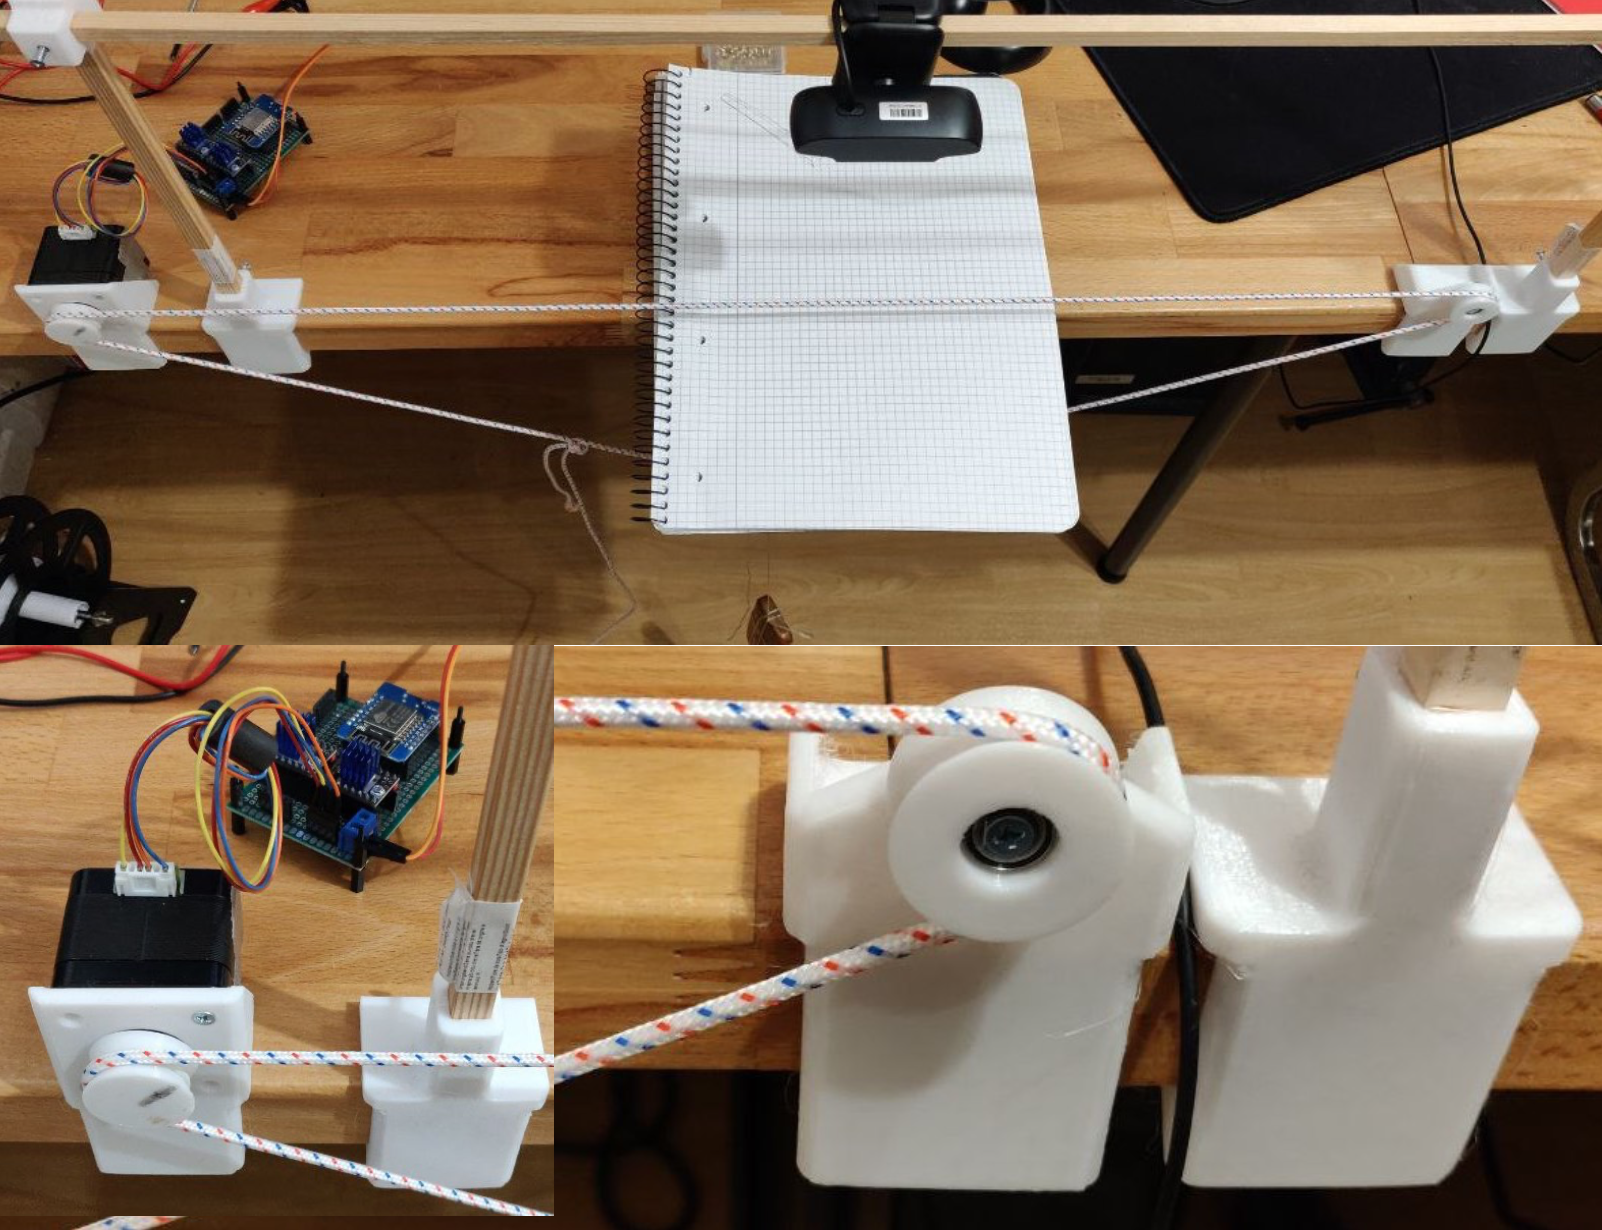
\includegraphics[width=10cm]{Abbildungen/testaufbau.png}
  \centering
  \caption{Die Gesamtansicht inklusive der Kamera, welche auf das Seil vor einheitlichem Hintergrund gerichtet ist (oben). Die Umlenkrolle mit Motor und Steuerung ist links zu sehen. Die Halterung für die Umlenkrolle und das Kameragestell sind rechts abgebildet. 
 }
  \label{fig:testaufbau}
\end{figure*}
	\subsection{Testaufbau}
	Der für die Entwicklung und Live Demonstration des linearen Encoders benötigte Datensatz wurde mithilfe eines für diesen Zweck dedizierten Testaufbaus aufgenommen, welcher in Abbildung \ref{fig:testaufbau} zu erkennen ist. Das Testen mit Videos erlaubt Softwareentwicklung ohne den Testaufbau live zu bedienen. Der Testaufbau besteht aus zwei stationären Halterungen, welche fest an einem Tisch angebracht werden können. Das Seil wird über zwei Umlenkrollen gespannt, welche drehbar an den Halterungen gelagert sind. Das Seil wird mittels eines Schrittmotors, welcher eine der beiden Rollen antreibt, in Bewegung versetzt. Schrittmotoren lassen sich genau positionieren und werden auch in CNC-Maschinen benutzt. Die Kamera wird stationär und senkrecht über dem Seil an einer Halterung befestigt. Diese ist höhenverstellbar. Das Sichtfeld der Kamera wird direkt auf das Seil ausrichtet.
	


	
	\subsubsection{Software}
	Für die Aufnahme der Videos wurde ein Python-Skript geschrieben. 
	Zuerst wird ein Thread für die Videoaufnahme gestartet. Dieser nimmt mit einer gegebenen Framerate Bilder auf und legt diese im Arbeitsspeicher ab. Für die Bildaufnahme wird das Paket \texttt{imageio} benutzt. Im Hauptthread wird eine angegebene Bewegungsfolge ausgeführt. Diese ist eine Folge von Tupeln aus Position, Geschwindigkeit und Verzögerung zur nächsten Bewegung. Für die Tests wurde sich wiederholt mit einer konstanten Geschwindigkeit zwischen zwei Positionen bewegt. Sind die Bewegungen ausgeführt, so werden die Bilder einzeln auf die Festplatte und auch als Video abgelegt. Im Test der Methode können die Bilder nun sequentiell mit \texttt{imageio} geladen werden.
	
	\subsubsection{Hardware}
    Die Ansteuerung des Motors wurde von einem privaten vorhergehenden Projekt übernommen. Ein ESP8266 Mikrocontroller empfängt und puffert über seinen seriellen Port einen Bytestream. Er erzeugt ein impulsartiges Signal für zwei TMC2208 - Schrittmotortreiber, welche den Strom für die Motoren schalten. In dieser Anwendung wurde jedoch nur einer benutzt. Für die Kommunikation zwischen dem Rechner und dem Mikrocontroller wurde ein selbst entwickeltes Protokoll benutzt. Dies erlaubt es, eine Schrittfolge, eine Rückmeldung über den Füllstand des Anweisungspuffers und ein Setzen der Verzögerung zwischen den Motorschritten zu übermitteln.
    Die Halterungen wurden in Autodesk Inventor gezeichnet, mit Ultimaker Cura zerteilt und dann 3D-gedruckt. Zu beachten, ist dabei das Durchrutschen der Seile, was allerdings über die insgesamt kleinen Distanzen der Tests vernachlässigbar ist.
    %bilder hinzufügen (Testaufbau/Mikrokontroller)
    
	%Felix
	%footage recorder
	%motor/steuerung
	
\begin{figure*}
  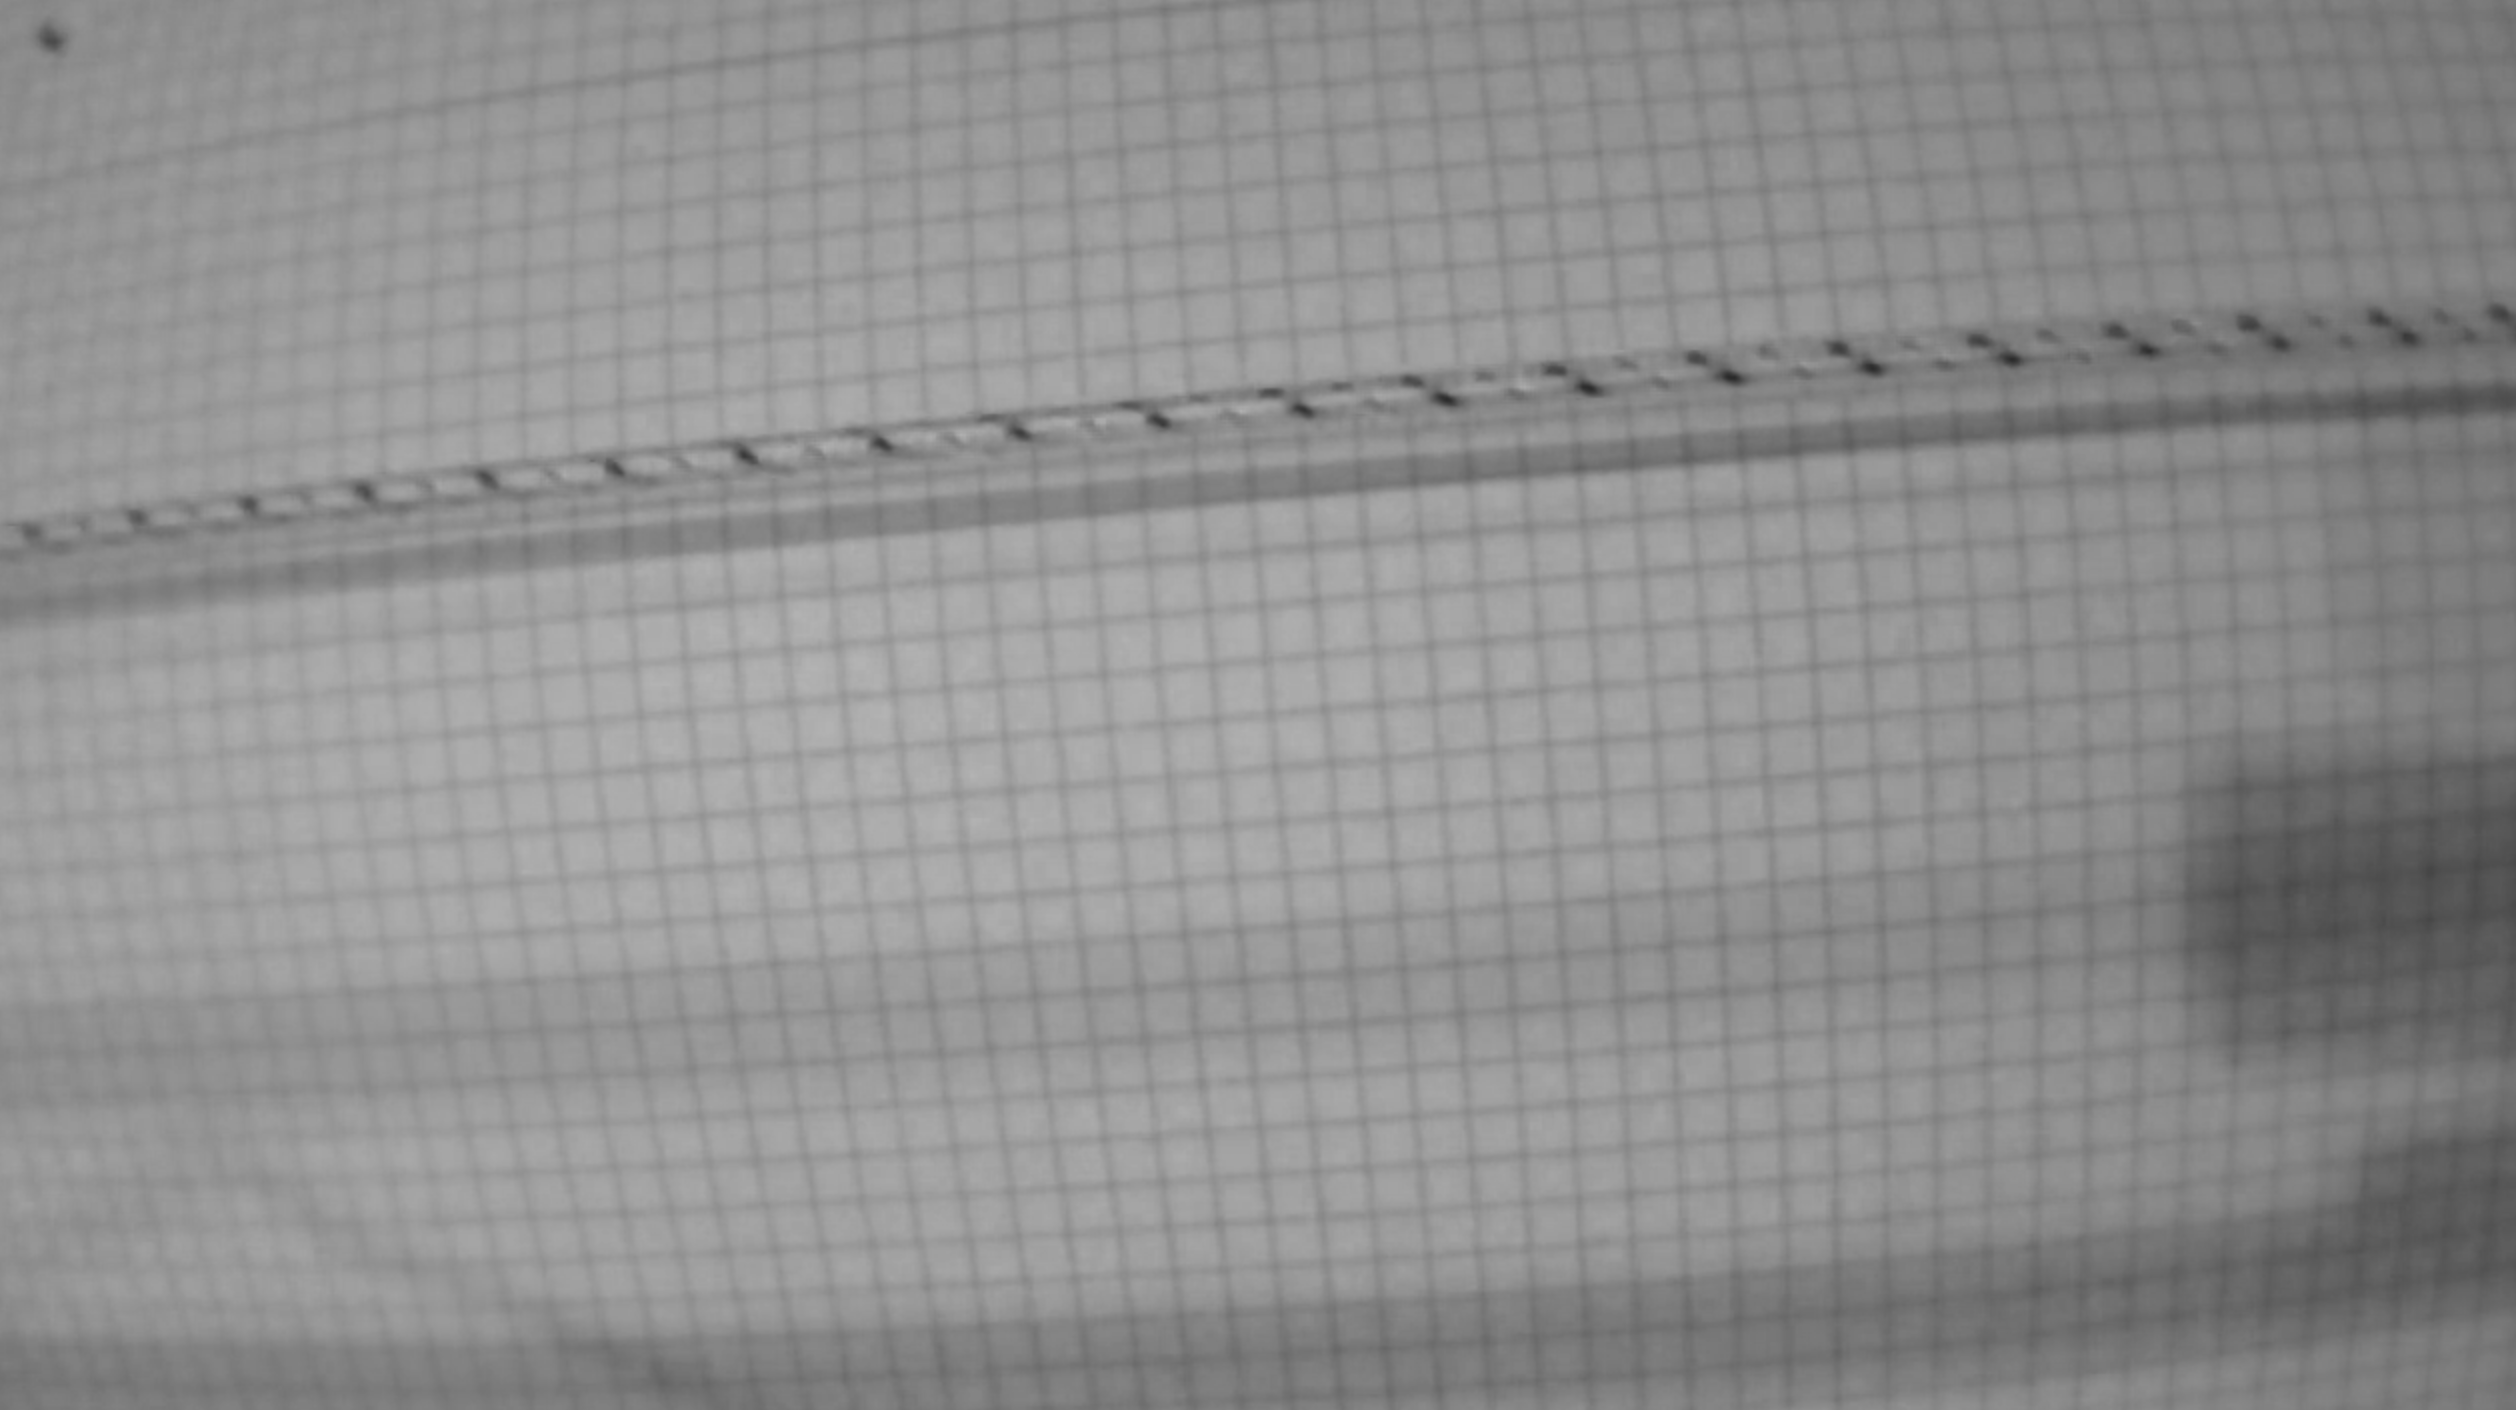
\includegraphics[width=10cm]{Abbildungen/image_frame.png}
  \centering
  \caption{Ein Frame der Testaufnahme \texttt{motor\_test\_1.mp4}
 }
  \label{fig:videoframe}
\end{figure*}
	\subsection{Datensatz}
	Die mit einer 30 FPS, 80° Weitwinkel-Webcam (RAPOO XW1701) aufgenommenen Testvideos des Seils sind mit 720p aufgelöst. Dies sorgt für eine verhältnismäßig niedrige Qualität des Videos. Die Aufnahmen sind des Weiteren verschwommen, verzeichnet und es sind Schatten auf dem Bild zu erkennen, wie in Abbildung \ref{fig:videoframe} zu sehen ist.
	Um diese trotzdem genau zu verarbeiten, muss unsere Methode robust sein. Zunächst wurden für die Entwicklung des linearen Encoders sechs verschiedene Testvideos aufgenommen. Diese unterscheiden sich in der Bewegung des Seils, sowie im Ausmaß der Störung des Bildes.
	

	
	%tabelle mit test parametern?
	%klingt nice aber eher in Evalutation oder?
	\subsection{Live-Demo}
	Für die Live-Demo wurde ein Testskript geschrieben, um die Funktionen der Bibliothek vorzuführen. Es erlaubt als Eingabe ein Video oder einen Stream von einer Webcam und erlaubt die Ausgabe von Zwischenschritten, das Ausprobieren der verschiedenen Methoden und auch einen geschlossenen Regelkreis mit dem Motor zu zeigen.
	
	\subsection{Anzeige der Messungen}
	Das Skript kann in einem Plot die gemessene Distanz über die Zeit ausgeben. Hierfür wurden zwei Varianten implementiert. In der ersten Variante wird abwechselnd die Distanz gemessen und das Ergebnis ausgegeben. Da die Ausgabe vor allem mit Debug-Ausgabe zeitintensiv ist, ist die Höchstgeschwindigkeit bei Echtzeit begrenzt. Im Gegenzug dafür wird jeder Messpunkt angezeigt.
	
	Alternativ wird ein Hintergrundthread gestartet, welcher die Bilder aus der Webcam zuschneidet und die Verschiebung bestimmt. Eine mit dem Thread geteilte Variable wird mit einem Lock geschützt und beinhaltet, jederzeit zugänglich die zuletzt bestimmte Position. Dies erlaubt die Messung kontinuierlich schnell durchzuführen, hat aber den Nachteil, dass die Updates nicht jede Messung zeigen. Da die gemessenen Werte jedoch vollständig als eine Reihe in der Debug-Information abgelegt sind, wird keine gemessene Position angezeigt.
	\subsubsection{Finden der Startposition}
	Um eine kleine Anwendung der Bibliothek zu demonstrieren, wurde die Webcam benutzt. Der Motor wird so angesteuert, dass er probiert, sich in die Startposition zurückzubewegen. Hierzu wird die Messung ebenfalls parallel im Hintergrund ausgeführt. Dies ist notwendig, da die Ansteuerung des Motors den aktuellen Thread blockiert, bis die Bewegung fertig ist. 
	Ein anderer Teil des Skripts erlaubt es eine bestimmte Anzahl an Schritten zu fahren, um für eine Kombination von Rollen und Seil das Verhältnis von Motorschritten, zu Seilperioden empirisch zu bestimmen. Dieses Verhältnis kann benutzt werden, um iterativ die gemessene Position in eine Anzahl von Schritten umwandeln und jeweils entgegengesetzt den Motor zu fahren, was einwandfrei funktioniert. Das Seil kann festgehalten, bewegt und teilweise verdeckt werden und trotzdem kehrt das Seil in die Startposition zurück. Probleme gab es, sobald das Seil zu weit senkrecht zu seiner Richtung verläuft oder wenn es zu schnell bewegt wird. Dies führt dazu, dass die diskrete Anzahl bewegter Perioden nicht der realen Bewegung entspricht. Es wird nun eine Position angefahren, welche eine diskrete Anzahl an Perioden neben der Startposition liegt. Die Genauigkeit zwischen den Perioden ist jedoch immer noch gut.
	
	%live demo beschreiben
    \subsection{Limitationen}
    Der lineare Encoder ist sowohl von der praktischen Seite als auch von der theoretisch Seite in seiner Fähigkeit, die Verschiebung eines Seiles zu bestimmen, beschränkt. Auf der praktischen Seite ist das System durch die benutzte Kamera und deren Bildrate sowie ihrer Auflösung beschränkt.\\
    
    Die theoretische Betrachtung zeigt, dass sich aus der Framerate der genutzten Kamera gemäß dem Nyquist-Shannon-Abtasttheorem eine Maximalgeschwindigkeit für das Seil ergibt. Dies äußert sich durch das Phase-Unwrapping. Ist die Bewegung größer als eine halbe Periode, kann nicht mehr eindeutig entschieden werden, ob sich vorwärts oder rückwärts bewegt wurde. Die Höchstgeschwindigkeit $v_{max}$ ergibt sich somit ausschließlich aus der Länge einer Periode $s_{period}$ und der Frequenz der Bildaufnahme $f_{framerate}$.
    \begin{equation}
    %f_{framerate}=2*f_{tag}\\
    v_{max}=\frac{s_{period}}{2}\frac{1}{f_{framerate}}
    \end{equation}
    Des Weiteren bringt das verwendete Seil Limitierungen mit sich. Zum einen ist zu beachten, dass die meisten handelsüblichen Seile zwar mit einem regelmäßigen Muster geliefert werden, dieses sich allerdings spiralförmig um das Seil windet. Spiralmuster haben dabei den Nachteil, dass sie bei einer Rotation des Seils um die eigene Achse die beobachtete Distanz verfälschen und damit unbrauchbar machen. %erklärung kurz
    Wir nehmen eine feste RoI an, d.\,h. das Seil darf sich nicht oder nur sehr geringfügig quer zur gemessenen Achse bewegen. Dies ist durch Verwendung eines einzelnen Referenzbildes bedingt. Das Referenzbild wird benutzt, um fortlaufend die Verschiebung in der Periode der Seilmarkierungen zu bestimmen. 
    %Für die Genauigkeit des Musters die Herstellerspezifikation zu beachten, da sich die Distanzmessung aus dem Abstand zweier Markierungen ergibt.
    Aus der Anzahl Perioden lässt sich ein Länge in Meter berechnen, es ist aber zu beachten, dass diese sich auch unter Belastung ausdehnen kann. Diese hängen unter anderem von Material und Herstellung des Seils ab. %Die Methode zählt die Distanz in Perioden auf dem Seil. Für die absolute Länge sind also auch Dehnbarkeit und Länge der Perioden zu beachten.
    %bruno
% wo stößt unser alg an die grenzen
% -RoI ist fix
% -wir haben ein base image / seil muss regelmäßig sein
% -seil drehen/gewundene muster
% framerate/periode seil => max geschwindigkeit
\section{Implementierung}
Im Kapitel Implementierung wird auf die Details der Implementierung des Prototyps sowie die anschließende Entwicklung der Software-Bibliothek eingegangen. 
\begin{figure*}
  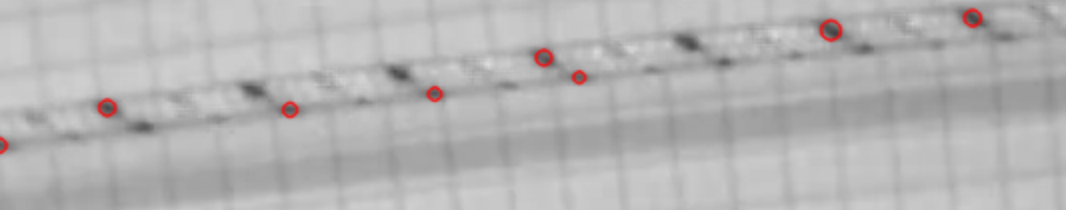
\includegraphics[width=10cm]{Abbildungen/blob_detection.png}
  \centering
  \caption{Die roten Kreise zeigen die erkannten ,,Blobs'' auf dem Seil.}
  \label{fig:blobImg}
\end{figure*}
\begin{figure*}
  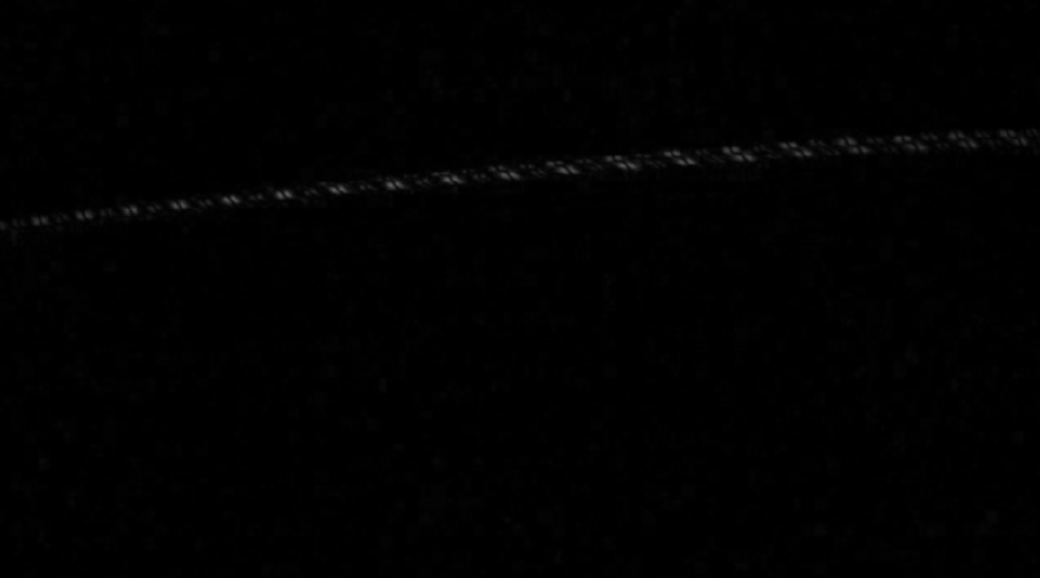
\includegraphics[width=10cm]{Abbildungen/diff_img_cropped.png}
  \centering
  \caption{Die Abbildung zeigt das Differenzbild aufeinander folgender Frames.}
  \label{fig:diffImg}
\end{figure*}

\subsection{Implementierung des Prototyps}
Der Prototyp sowie die Software-Bibliothek werden in der Programmiersprache Python umgesetzt, dabei wird der Codestil PEP-8 verwendet, um den Programmcode übersichtlich und einheitlich zu gestalten.
Für die Kollaboration bei der Implementierung des Projekts wird das Versionierungssystem git sowie die Plattform GitHub genutzt. Der Git-Workflow des Repositorys wird durch die Nutzung von Feature-Branches umgesetzt. \\
Wie in Abschnitt \ref{RoI_Extraktion} beschrieben, lag der Fokus der initialen Prototypentwicklung auf der Extraktion der RoI. Dazu wurden zunächst verschiedenste OpenCV\footnote{\url{https://opencv.org}} Funktionen
wie z.\,B. die Blob-Detektionsfunktion  \texttt{cv2.SimpleBlobDetector} \footnote{\url{https://docs.opencv.org/3.4/d0/d7a/classcv_1_1SimpleBlobDetector.html}} benutzt, um das Muster des Seils zu erkennen, wie in Abbildung \ref{fig:blobImg} zu sehen ist.
Diese wurde in Verbindung mit diversen morphologischen Operationen und Schwellwertoperationen getestet, wie in einem Tutorial von Rosenbrock\footnote{\url{https://pyimagesearch.com/2016/10/31/detecting-multiple-bright-spots-in-an-image-with-python-and-opencv/}} beschrieben. Diese Methode hat sich allerdings, wie in Abbildung \ref{fig:blobImg} zu erkennen, als wenig robust erwiesen. 
Darüber hinaus wurden Differenzbilder für die RoI-Erkennung in Erwägung gezogen, wie in Abbildung \ref{fig:diffImg} zu sehen ist. Dieser Ansatz wurde allerdings auch verworfen, da die RoI vor der Erkennung der Bewegung vorliegen muss und zu diesem Zeitpunkt kein signifikantes Differenzbild existieren kann, da sich das Seil in Ruhe befindet.    
%Differenzbilder werden benutzt, irgendwo erklären

Als zuverlässigerer Ansatz hat sich die Anwendung des Canny-Algorithmus, siehe Abbildung \ref{CannySubsection}, welcher in OpenCV mit  \texttt{cv2.Canny()}\footnote{\url{https://docs.opencv.org/3.4/da/d22/tutorial_py_canny.html}} implementiert ist, herausgestellt.
Dieser wird in Verbindung mit der Hough-Transformation \ref{Hough_Transformation}, welche mittels  \texttt{cv2.HoughLines}\footnote{\url{https://docs.opencv.org/3.4/d9/db0/tutorial_hough_lines.html}} aufgerufen wird, für die Linienerkennung verwendet.
Anschließend wird das Fenster der RoI, wie in \ref{RoI_Ausschneiden} beschrieben, extrahiert. 

\begin{figure*}
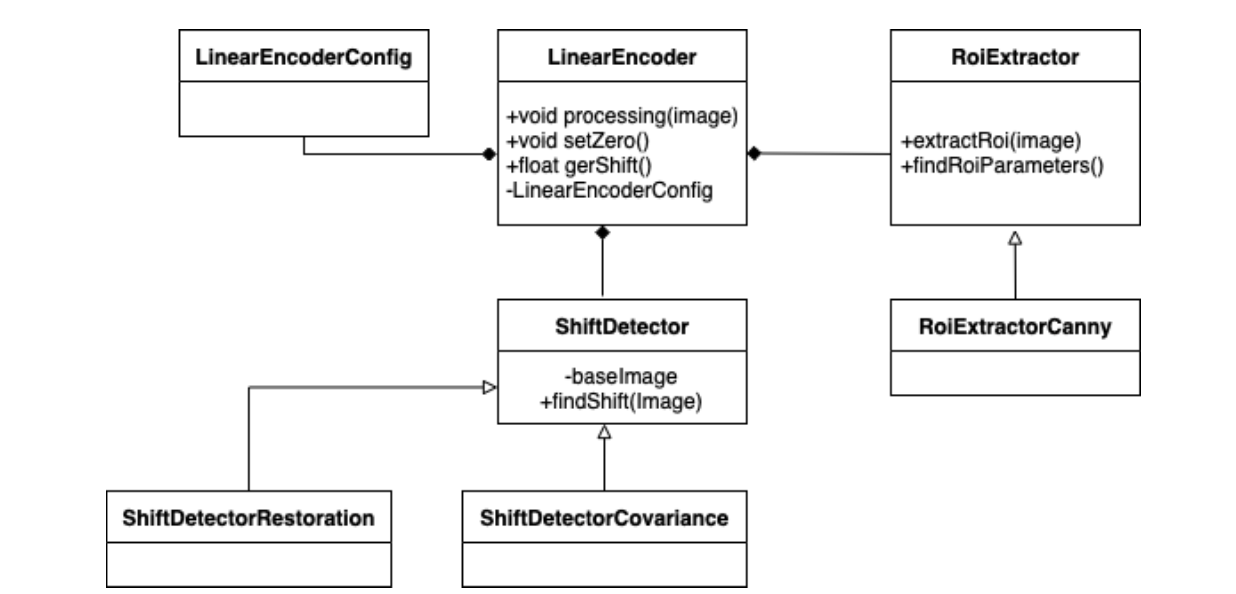
\includegraphics[width=10cm]{Abbildungen/KlassendiagrammWhiteBackground.png}
  \centering
  \caption{Das Klassendiagramm des linearen Encoders.}
  \label{fig:Klassendiagramm}
\end{figure*}

\subsection{Implementierung der Software-Bibliothek}
Nachdem die prototypische Umsetzung des linearen Encoders vollständig funktioniert hat, wurde mit der Refaktorisierung begonnen. Dazu wurden Python-Klassen für die RoI-Extraktion und die Verschiebungserkennung erstellt. Dort werden dem Benutzer der Software-Library zwei Möglichkeiten zur Verfügung gestellt. Zum einen kann die Verschiebung mittels Korrelation (siehe Abschnitt \ref{Autokorrelation}) und zum anderen mittels Restauration (siehe Abschnitt \ref{Shift_detection_by_Restoration}) bestimmt werden. Des Weiteren sollen die Parameter des linearen Encoders möglichst einfach zugänglich gemacht werden, was durch die Konfigurationsklasse erreicht wird. %implementation?

In Abbildung \ref{fig:Klassendiagramm} ist das vollständige Klassendiagramm dargestellt. Zusätzlich wird dem Projekt eine \texttt{setup.cfg} Datei beigefügt, welches die Metadaten des Projektes enthält und eine \texttt{pyproject.toml} Datei angelegt, welche für das Setup des Projekts in Pycharm zuständig ist. Außerdem wurde eine \texttt{LICENSE} Datei, welches eine übliche MIT-License Lizenzerklärung enthält und eine \texttt{README.md} hinzugefügt, welche eine grundsätzliche Dokumentation zur Benutzung und Funktionsweise des linearen Encoders enthält.

\subsubsection{Verwendetete Bibliotheken}
Für RoI-Extraktion wurde vorwiegend die \texttt{OpenCV}-Bibliothek benutzt, da diese eine Vielzahl an Methoden zur Bildverarbeitung bereitstellt. Die Eingabe und Ausgabe von Bildern und Videos erfolgt mithilfe von \texttt{imageio}. Diese Software-Bibliothek erlaubt den einfachen Zugriff auf die erste angeschlossene Webcam. Für die Implementierung der Verschiebungserkennung wurden hauptsächlich \texttt{SciPy} und \texttt{NumPy} benutzt, da sie Methoden für die fast Fourier-Transfromation (FFT) und Kreuzkorrelation bereitstellen. Zum Anzeigen der Ergebnisse wurde \texttt{matplotlib} benutzt.

\subsubsection{Debug Output}
Da der Algorithmus sehr viele Schritte hat und es nicht direkt ersichtlich ist, was in jedem Schritt geschieht, wurden Zwischenergebnisse als Bilder und Datenreihen in einem Dictionary in dem jeweiligen Objekt abgelegt. Nach dem Ausführen einer Funktion wie z.\,B. RoI bestimmen oder Verschiebung berechnen, können in dem Verzeichnis alle Zwischenergebnis unter ihrem Namen gefunden werden. Dies erlaubt es in der Live-Demo, Schritt für Schritt den Algorithmus zu zeigen. Außerdem ist die parallele Ausführung im Hintergrund möglich, ohne \texttt{Matplotlib} auf dem Hintergrundthread auszuführen. Das Ablegen der Zwischenergebnisse kann mit einer Klassenvariable aktiviert werden.

\section{Evaluation}
Für die Evaluation der Funktionstüchtigkeit des linearen Encoders werden zuerst quantitativ Evaluationsmetriken definiert, um anschließend deren Ergebnisse qualitativ einzuordnen. 

%nach mit hilfe/mithilfe schauen

\subsection{Experiment zur Genauigkeit}
Es wurde ein Experiment durchgeführt, um die Robustheit und Genauigkeit der Methode zu testen. Die Idee war es hierbei, mithilfe des Testaufbaus wiederholt mit dem Schrittmotor eine Bewegung auszuführen, welche die Antriebsrolle am Ende zu ihrer Null-Position zurückkehren lässt. Diese Bewegung des Motors wurde so gewählt, dass das Seil möglichst viel in eine Richtung durchrutscht. Dies wurde durch viele plötzliche Stopps in eine Richtung, aber eine durchgängige Bewegung in die andere Richtung erreicht. Ein Zyklus dieser Bewegung ist in Abbildung \ref{fig:zyklus} zu sehen, die Wartezeiten zwischen den Schritten sind jedoch von $0,1$ Sekunde auf $1$ Sekunde erhöht, damit die Treppenstruktur ersichtlich wird.

\begin{figure*}
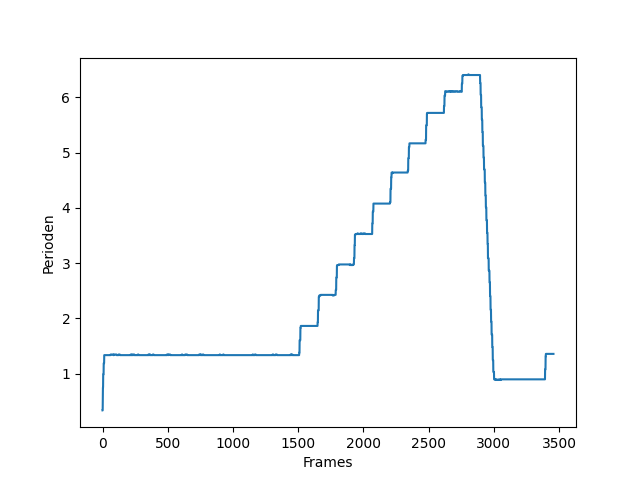
\includegraphics[width=10cm]{Abbildungen/Bewegungszyklus.png}
  \centering
  \caption{Ein Zyklus der Testbewegung.}
  \label{fig:zyklus}
\end{figure*}
Dieser Bewegungszyklus ist nun 100 Mal wiederholt worden und nach jedem Zyklus wurde die gemessene Verschiebung geloggt. Im zweiten Versuch wurde anschließend die gemessene Verschiebung mit dem Motor in die entgegengesetzte Richtung gefahren und ist erneut gemessen worden. Es ergeben sich drei Datenreihen, die in Abbildung \ref{fig:measured} zu sehen sind.  Die Ausführung der 100 Zyklen hat ca. 5 Minuten gedauert.
\begin{figure*}
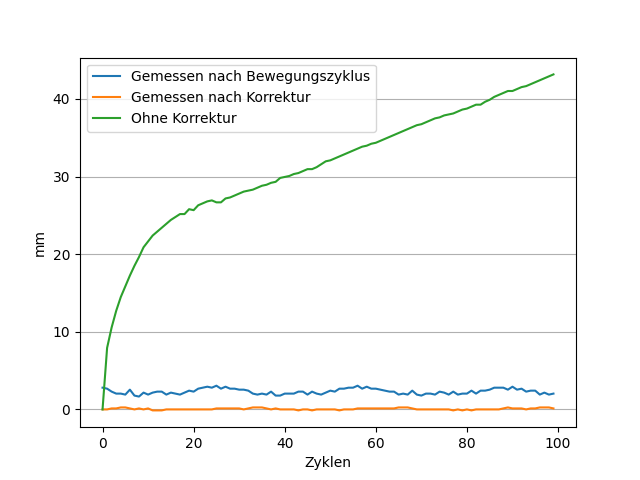
\includegraphics[width=10cm]{Abbildungen/Testergebnisse_durchrutschen.png}
  \centering
  \caption{Vom Algorithmus gemessene Verschiebungen}
  \label{fig:measured}
\end{figure*}
Es lässt sich insgesamt sehen, dass unsere Methode über lange Zeiträume zuverlässig  die Position des Seiles akkurat messen kann.

Abschließend wurde mithilfe einer Nadel durch das Seil und einem fest angebrachten Lineal die tatsächliche finale Verschiebung gemessen. Ohne Korrektur wurde eine finale Verschiebung von $43$ mm gemessen, verglichen mit $43.16$ mm berechnet aus der in Perioden gemessenen Verschiebung und dem bekannten Verhältnis Millimeter pro Periode. Dieses wurde berechnet, indem mit einem Lineal fünf Perioden als $56$ mm gemessen wurden. 
Bei dem Versuch mit laufender Korrektur war die finale Abweichung zu klein, um sie zuverlässig an dem Lineal abzulesen.

\subsection{Evaluation und Diskussion}
Grundsätzlich lässt sich sagen, dass das implementierte lineare Encoder System in der Lage ist, die Bewegung eines Seils verlässlich zu bestimmen. Des Weiteren ist der lineare Encoder robust gegenüber kleineren Störungen im Bild, die nicht direkt die RoI betreffen. Die RoI kann auch dann noch bestimmt werden, wenn Teile des restlichen Bildes nicht flach sind, wie in der Aufnahme \texttt{motor\_test\_6.mp4} demonstriert wird, wenn die RoI dynamisch bestimmt wird. Außerdem konnte auch eine Robustheit gegenüber Belichtungsänderungen festgestellt werden. Das bedeutet, dass das System funktionstüchtig bleibt, solange der Kontrast der Aufnahme die Verschiebungserkennung der Seilmarkierungen zulässt.
Demzufolge ist das System zuverlässig genug, um in andere Anwendungen integriert zu werden. Vorher könnten noch ein einige Quality of Life Changes gemacht werden, wie z.\,B. die Auslieferung als Python Paket und eingebautes Multithreading.

\section{Ausblick}
Das entwickelte lienare Encodersystem entspricht der in Abschnitt \ref{Zielsetzung} geforderten Zielsetzung, trotzdem konnten wir einige Verbesserungsvorschläge identifizeiren. Die folgenden Verbesserungen erachten wir als besonders wichtig: die Fähigkeit des linearen Encoders, die RoI dynamisch, das heißt während des Betriebs, zu bestimmen. Des Weiteren ist Robustheit gegenüber Axial-Rotation des Seils wünschenswert. Diese lässt sich softwareseitig allerdings nur schwer implementieren, im Gegensatz dazu ließe sich das spiralmarkierte Seil durch ein ringmarkiertes Seil ersetzen. 

Das Ausschneiden der RoI kann optimiert werden, da zurzeit erst das ganze Bild gedreht und anschließend zugeschnitten wird. Wenn die Affine Transformation und die Interpolation direkt in einem Schritt implementiert werden, kann der Rechen-Overhead für jeden Frame reduziert werden.

 Eine zusätzliche Erweiterung wäre die Fähigkeit des linearen Encoders, mehrere Seile in einer Aufnahme gleichzeitig zu verarbeiten. Dies hat zusätzlich den Vorteil, dass Aufnahmen, in denen mehrere Seile zu erkennen sind, nicht zu Fehlern aufgrund von Ambivalenz führen.

Auf der Software-Seite ist es mit steigender Komplexität der linearen Encoder Softwarebibliothek folglich unabdingbar, zukünftig fehlerhaftes Verhalten besser handzuhaben und entsprechend mehr Exception-Handling zu implementieren. Außerdem wäre es möglich, eine schnellere Implementation zu schreiben. Hierzu könnten C++ und Cython benutzt werden, um ein Python-Modul zu schreiben.
Voraussichtlich werden sich aus der Integrierung des linearen Encoders in den im Abschnitt \ref{Motivation} motivierten V-Plotter ergeben weitere sinnvolle Verbesserungen ergeben.
%maschienen/roboter damit bauen
%mehr robustheit
%schlaueres phase unwrappig

\appendix

\bibliography{AWP3Dbib}

\end{document}                          
